\documentclass[article]{memoir}

\usepackage{tikz}
\usetikzlibrary{positioning}


\begin{document}

\chapter{Overall structure}
\begin{figure}[htbp]
	\centering
	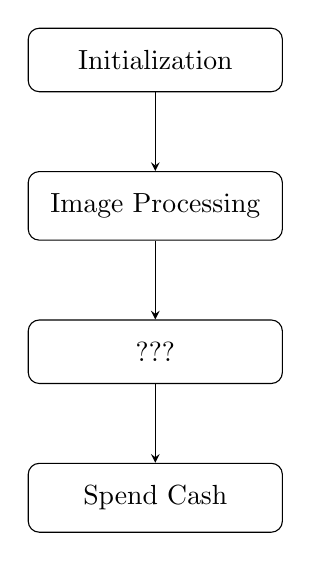
\begin{tikzpicture}
		\tikzset{module/.style={draw,
								rectangle,
								rounded corners,
								inner sep=8pt,
								text width=width("Image Processing"),
								align=center},
				 arrow/.style={->,
							   >=stealth}}
		% Nodes
	    \node[module] (init) {Initialization};
	    \node[module, below=of init] (image) {Image Processing};
	    \node[module, below=of image] (learning) {???};
	    \node[module, below=of learning] (win) {Spend Cash};
	    
	    % Arrows
	    \draw[arrow] (init) -- (image);
	    \draw[arrow] (image) -- (learning);
	    \draw[arrow] (learning) -- (win);
	\end{tikzpicture}
\end{figure}


\chapter{Code modules}
\section{Initialization}
\begin{figure}[htbp]
	\centering
	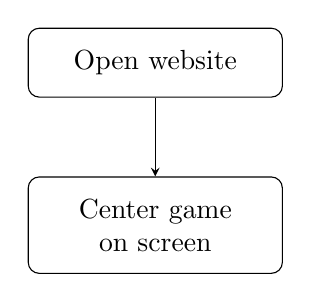
\begin{tikzpicture}
	\tikzset{module/.style={draw,
				rectangle,
				rounded corners,
				inner sep=8pt,
				text width=width("Image Processing"),
				align=center},
			arrow/.style={->,
				>=stealth}}
	% Nodes
	\node[module] (open) {Open website};
	\node[module, below=of open] (center) {Center game on screen};
	
	% Arrows
	\draw[arrow] (open) -- (center);
	\end{tikzpicture}
\end{figure}


\section{Image processing}

Haha


\end{document}
